\subsubsection{NASA-TLX}
\label{subsubsec:results_nasa_tlx_2}

\paragraph*{Analysis of the mental demand scale}\mbox{}\\

Figures \ref{fig:boxplot_noBase_md_4_scene} and \ref{fig:boxplot_noBase_md_4_rounds} presents the box plot for both groups, organized by the methods and the rounds. The mental demand is systematically higher for sighted people, which is expected. However, while blind participants considered the audio method less demanding, sighted participants prefered to the virtual cane. For both groups, we observe a decrease in the mental demand.

\begin{figure}[!htb]
    \centering
    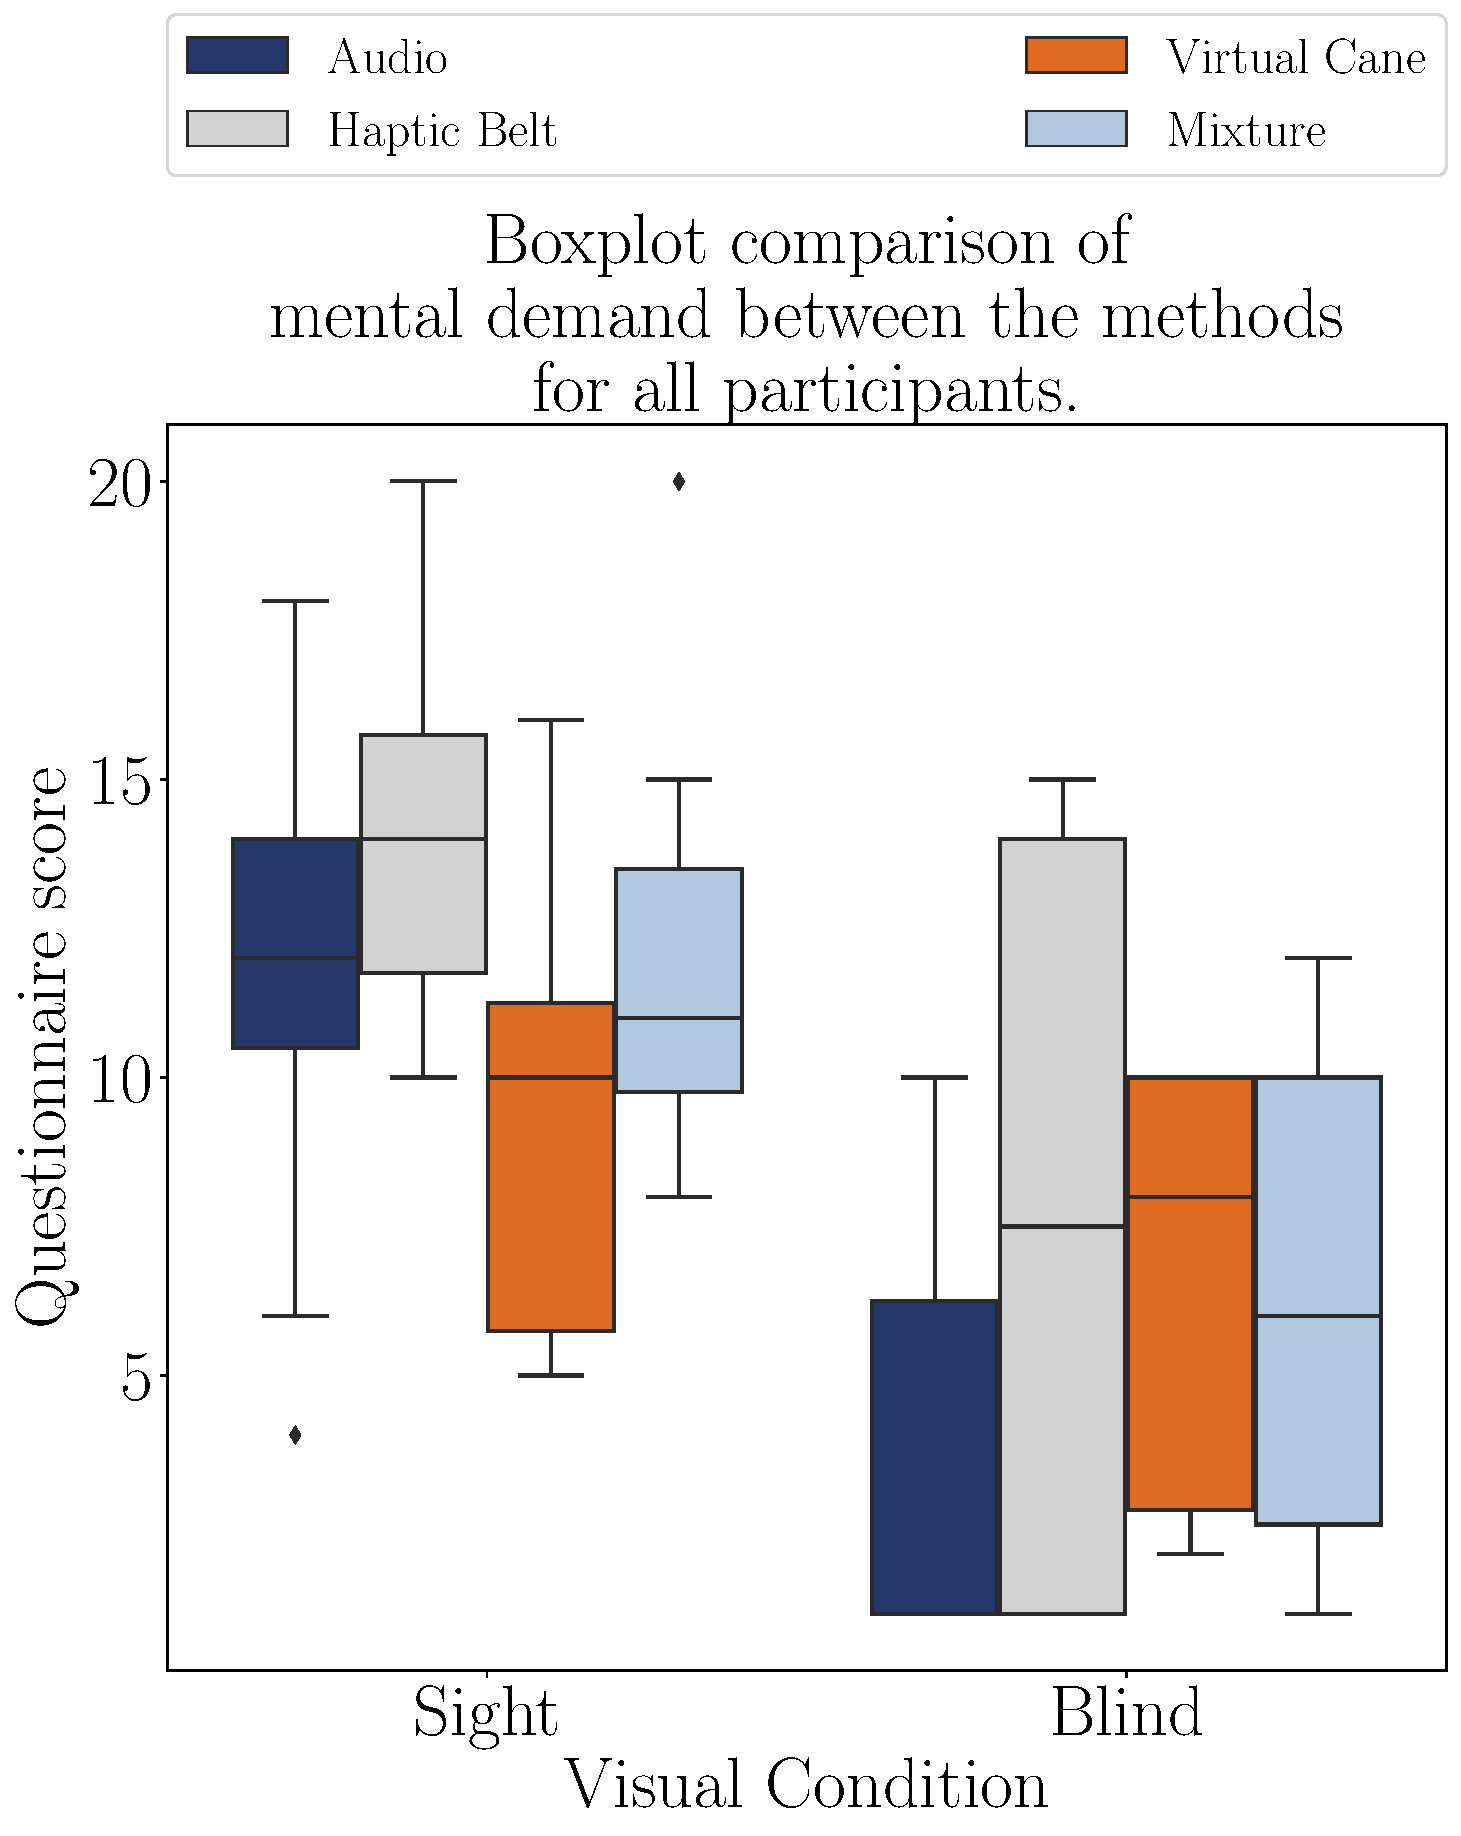
\includegraphics[width = 0.75\linewidth]{3 - Resultados/Figuras/boxplot_noBase_md_4_scene.pdf}
    \caption{Boxplot of the mental demand of the participants grouped by the methods.}
    \label{fig:boxplot_noBase_md_4_scene}
\end{figure}
\begin{figure}[!htb]
    \centering
    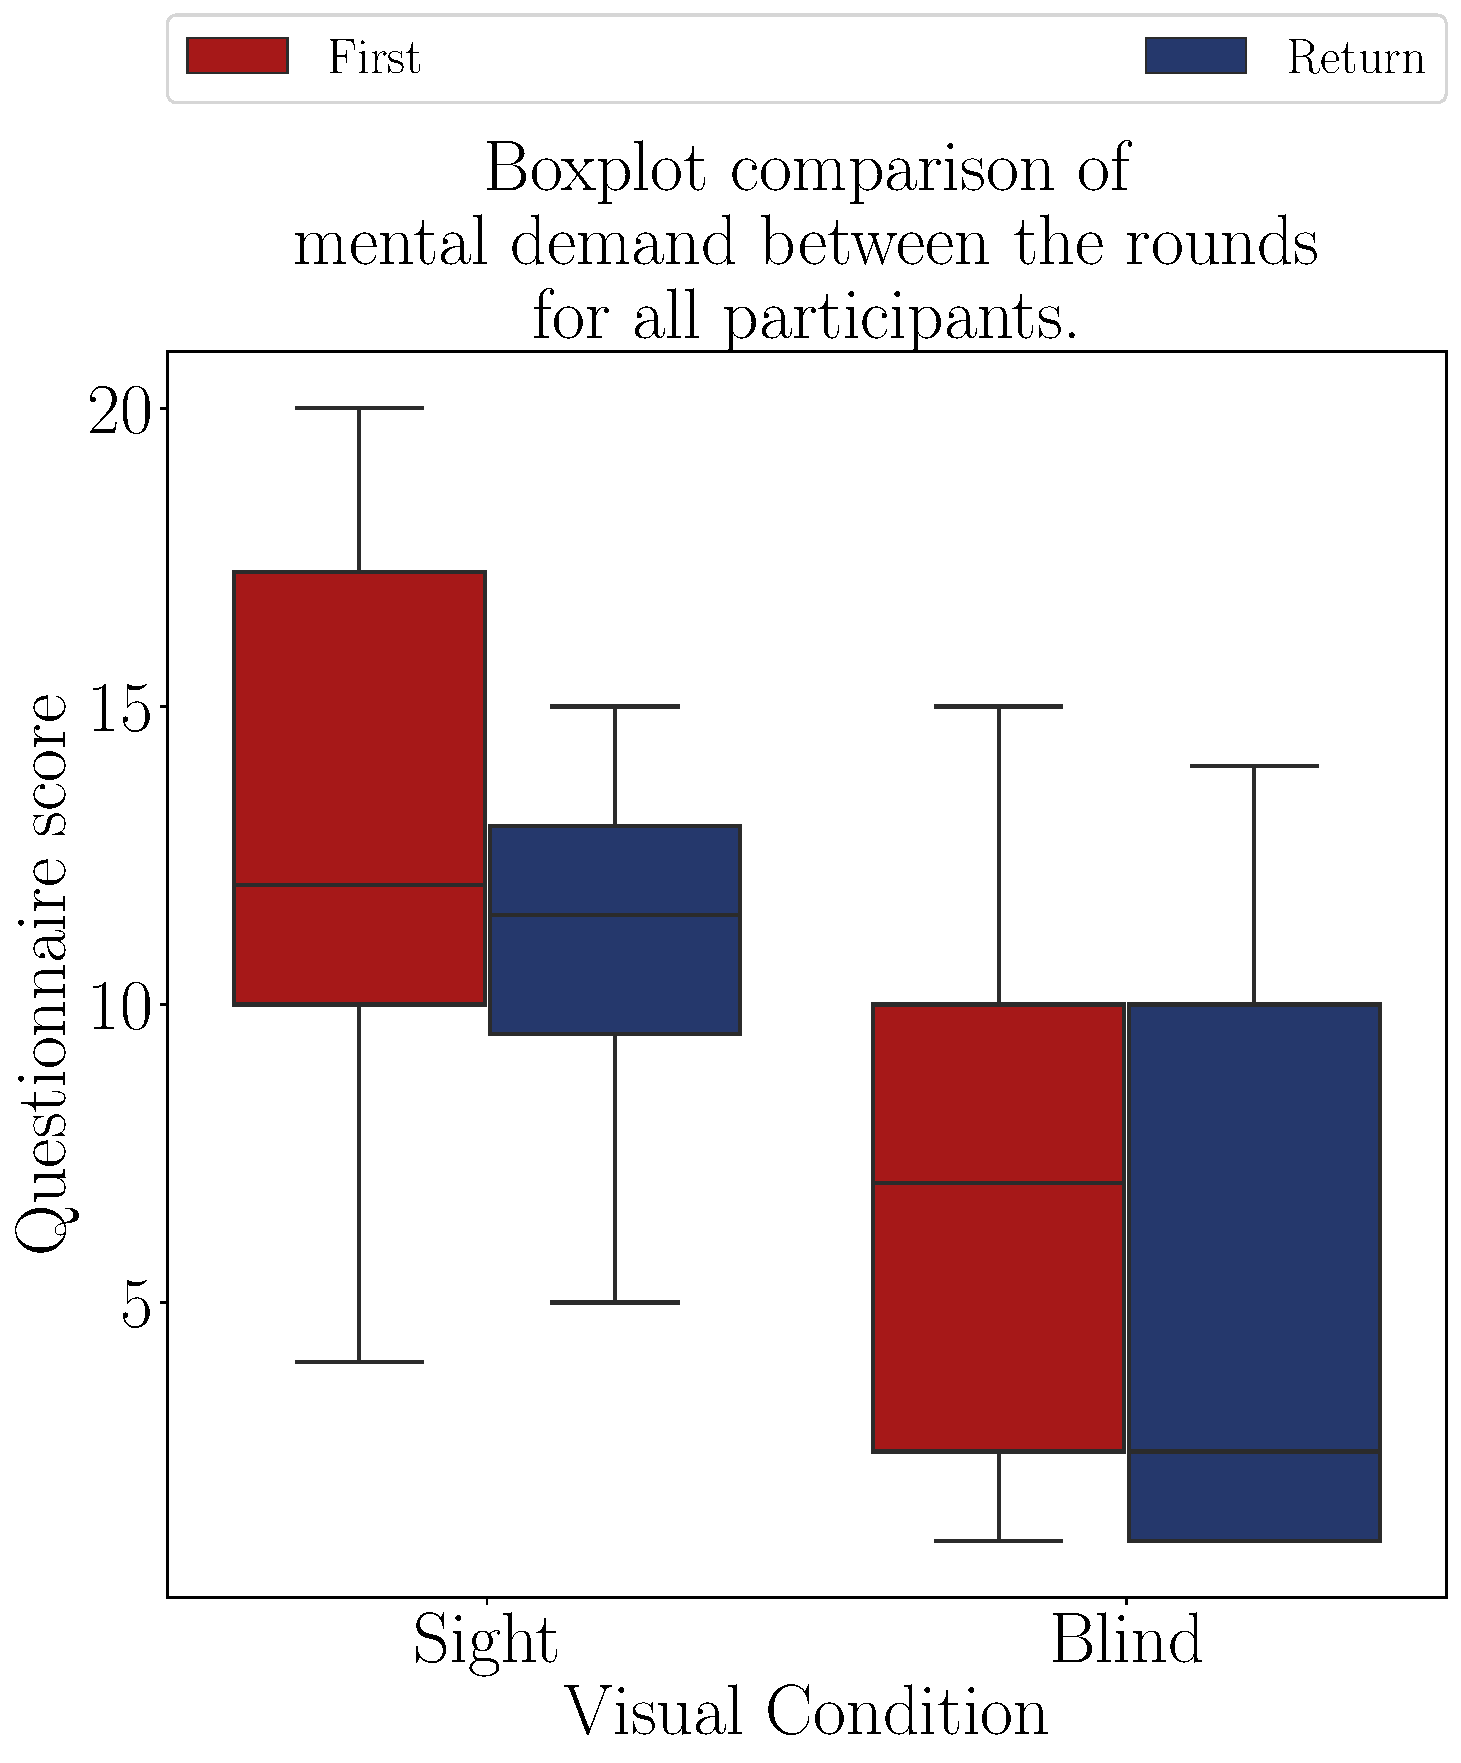
\includegraphics[width = 0.75\linewidth]{3 - Resultados/Figuras/boxplot_noBase_md_4_rounds.pdf}
    \caption{Boxplot of the mental demand of the participants grouped by the rounds.}
    \label{fig:boxplot_noBase_md_4_rounds}
\end{figure}

Table \ref{tab:blocanova_md_avg_two_way_blind_sight} brings the results of ANOVA. Unlike the blind participants, in the case of sighted ones, the p-value for the methods is below the threshold of 0.05, confirming it as a significant variable for the mental demand. In the case of the rounds, the data from both sighted and blind participants resulted in the exact p-value of 0.075, which is close to the traditional threshold of 0.05 but slightly higher. 

\begin{table}[!htb]
    \caption{Anova p-value for the mental demand average on each method'}
    \label{tab:blocanova_md_avg_two_way_blind_sight}
\begin{minipage}{0.45\linewidth}
    \subcaption{Blind participants}
    
\centering
\begin{tabular}{ll}
\toprule
          Source & P-Value \\
\midrule
    \    Methods &   0.170 \\
     \    Rounds &   0.075 \\
\    Interaction &   0.993 \\
\bottomrule
\end{tabular}

\end{minipage}%
\begin{minipage}{0.05\linewidth}
    \hfill
\end{minipage}%
\begin{minipage}{0.45\linewidth}
    \subcaption{Sight participants}
    
\centering
\begin{tabular}{ll}
\toprule
          Source & P-Value \\
\midrule
    \    Methods & 0.049** \\
     \    Rounds &   0.075 \\
\    Interaction &   0.990 \\
\bottomrule
\end{tabular}
    
\end{minipage}
\end{table}


%%%%%%%%%%%%%%%%%%%%%%%%%%%%%%%%%%%%%%%%%%%%%%%%%%%%%%%%%%%%%%%%%%%%%%%%%%%%
%%%%%%%%%%%%%%%%%%%%%%%%%%%%%%%%%%%%%%%%%%%%%%%%%%%%%%%%%%%%%%%%%%%%%%%%%%%%
%%%%%%%%%%%%%%%%%%%%%%%%%%%%%%%%%%%%%%%%%%%%%%%%%%%%%%%%%%%%%%%%%%%%%%%%%%%%
%%%%%%%%%%%%%%%%%%%%%%%%%%%%%%%%%%%%%%%%%%%%%%%%%%%%%%%%%%%%%%%%%%%%%%%%%%%%


\paragraph*{Analysis of the NASA-TLX score}\mbox{}\\

Figures \ref{fig:boxplot_noBase_nasa_4_scene} and \ref{fig:boxplot_noBase_nasa_4_rounds} present the boxplots of the NASA-TLX global score. Again, it is possible to see that sighted people usually give higher workload scores than blind ones. The influence of the round is approximately the same. However, the order of preference of the methods is different.

\begin{figure}[!htb]
    \centering
    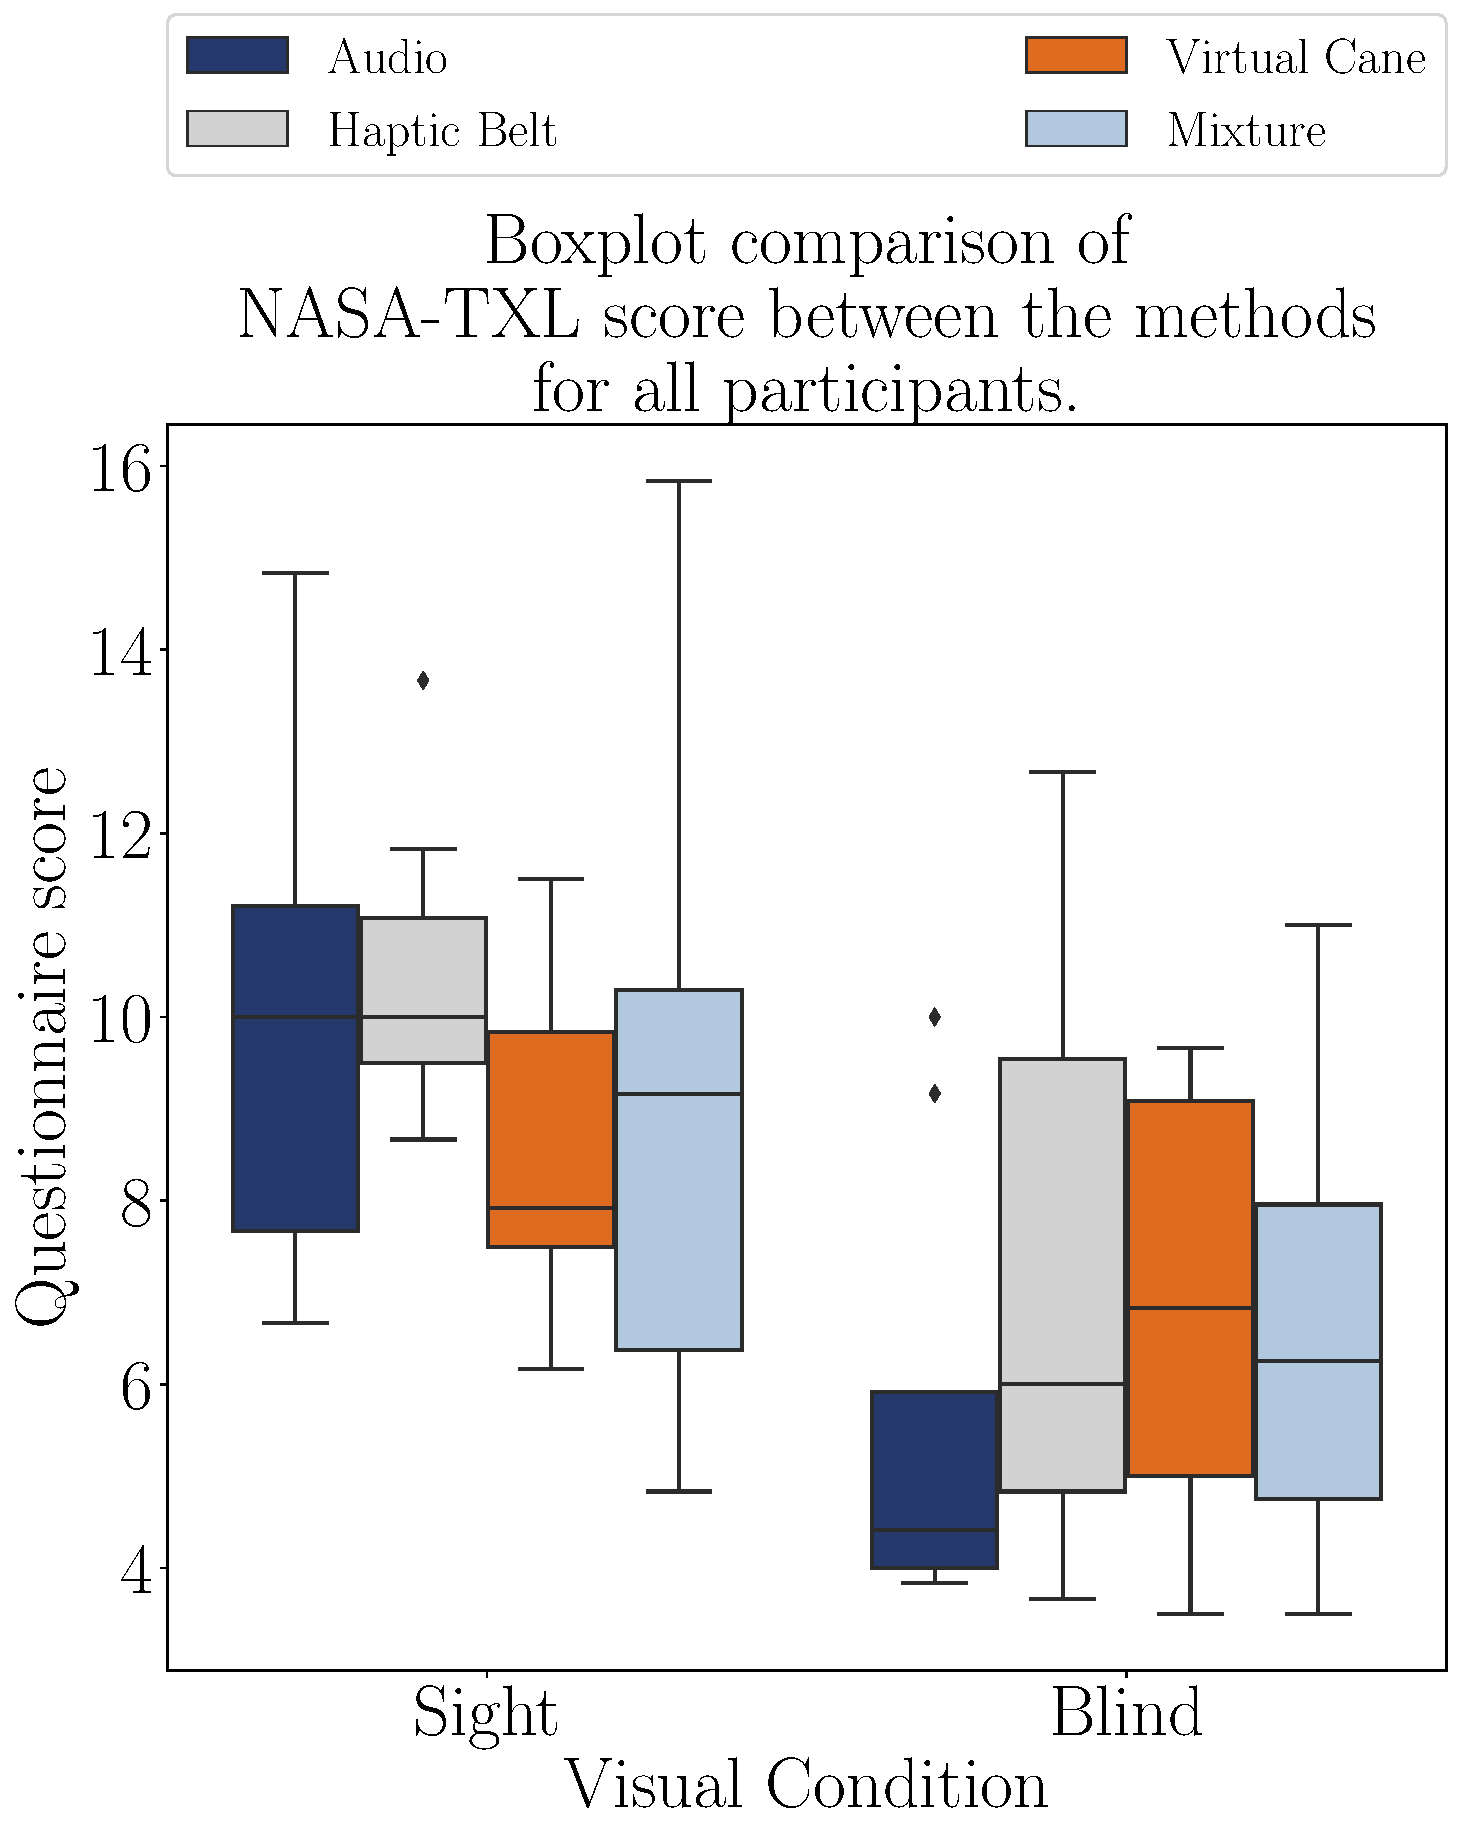
\includegraphics[width = 0.75\linewidth]{3 - Resultados/Figuras/boxplot_noBase_nasa_4_scene.pdf}
    \caption{Boxplot of the NASA-TLX score of the participants grouped by the methods.}
    \label{fig:boxplot_noBase_nasa_4_scene}
\end{figure}
\begin{figure}[!htb]
    \centering
    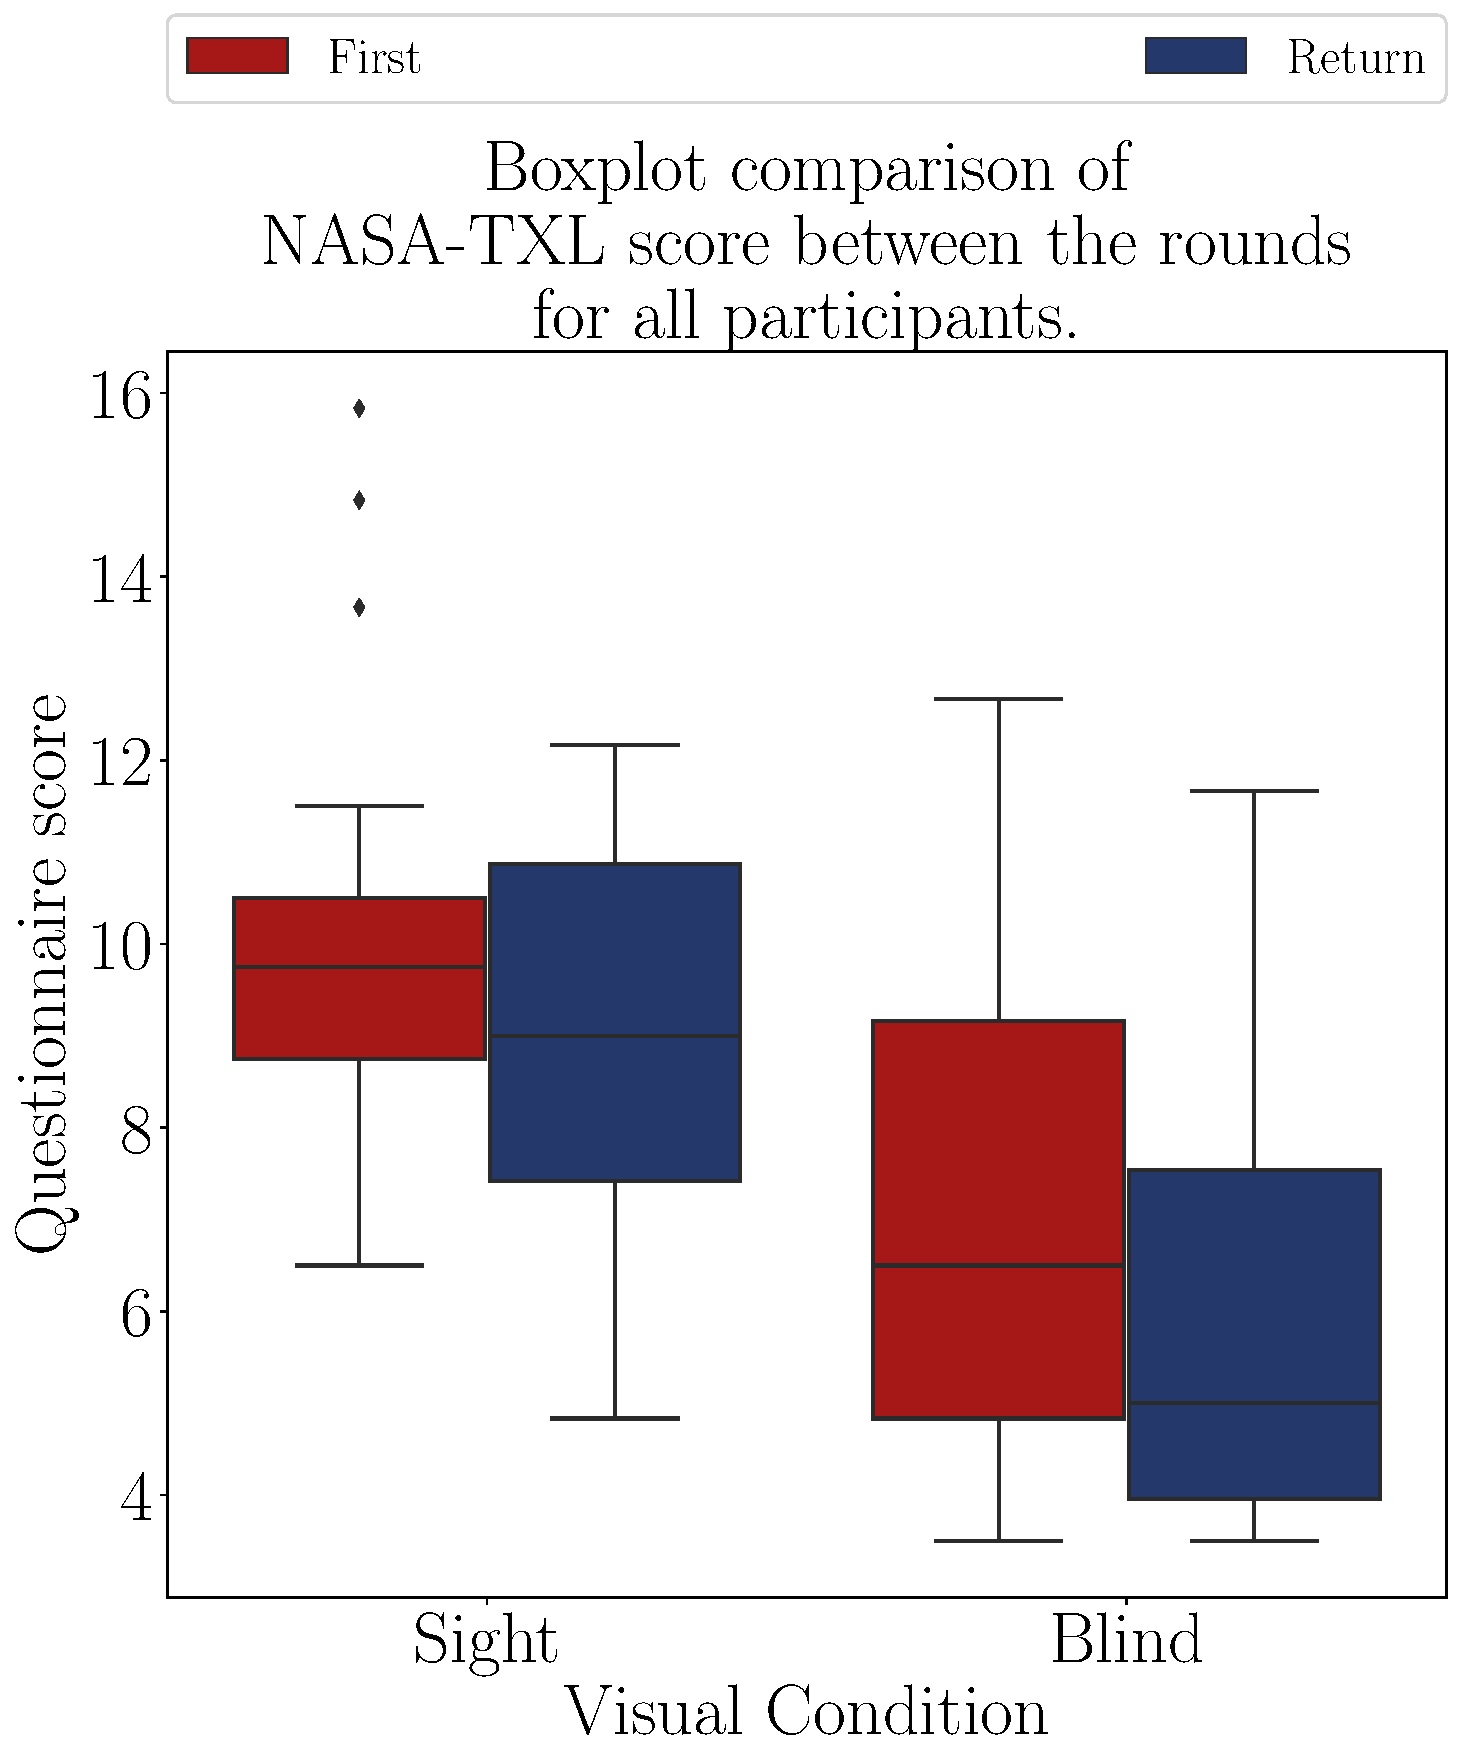
\includegraphics[width = 0.75\linewidth]{3 - Resultados/Figuras/boxplot_noBase_nasa_4_rounds.pdf}
    \caption{Boxplot of the NASA-TLX score of the participants grouped by the rounds.}
    \label{fig:boxplot_noBase_nasa_4_rounds}
\end{figure}

The p-values for both groups are presented in Table \ref{tab:blocanova_nasa_avg_two_way_blind_sight}. It confirms the influence of the round for both sighted and blind people. In the case of the methods, the p-value of blind is lower than the threshold of 0.5, while that of sighted is slightly higher.

\begin{table}[!thb]
    \caption{Anova p-value for the NASA-TLX score on each method}
    \label{tab:blocanova_nasa_avg_two_way_blind_sight}
    \begin{minipage}{0.45\linewidth}
        \subcaption{Blind participants}
        
\centering
\begin{tabular}{ll}
\toprule
          Source & P-Value \\
\midrule
    \    Methods & 0.029** \\
     \    Rounds & 0.022** \\
\    Interaction &   0.814 \\
\bottomrule
\end{tabular}

    \end{minipage}%
    \begin{minipage}{0.05\linewidth}
        \hfill
    \end{minipage}%
    \begin{minipage}{0.45\linewidth}
        \subcaption{Sight participants}
        
\centering
\begin{tabular}{ll}
\toprule
          Source & P-Value \\
\midrule
    \    Methods &   0.086 \\
     \    Rounds & 0.034** \\
\    Interaction &   0.688 \\
\bottomrule
\end{tabular}
    
    \end{minipage}
\end{table}